% Draft caption for the method figure (Fig. 2).  Usage in sections/method.tex:
%   \begin{figure*}[t]\centering
%     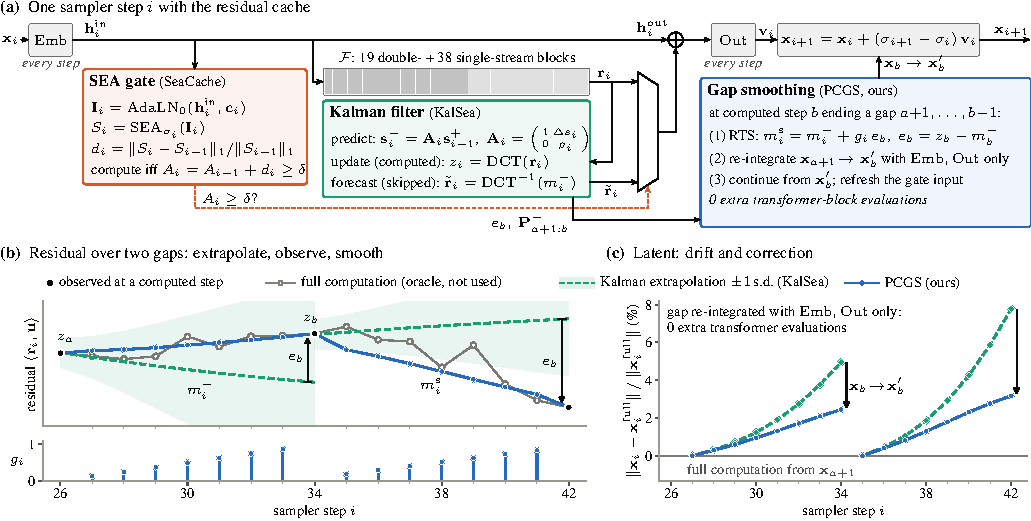
\includegraphics[width=\textwidth]{figures/method.pdf}
%     % Draft caption for the method figure (Fig. 2).  Usage in sections/method.tex:
%   \begin{figure*}[t]\centering
%     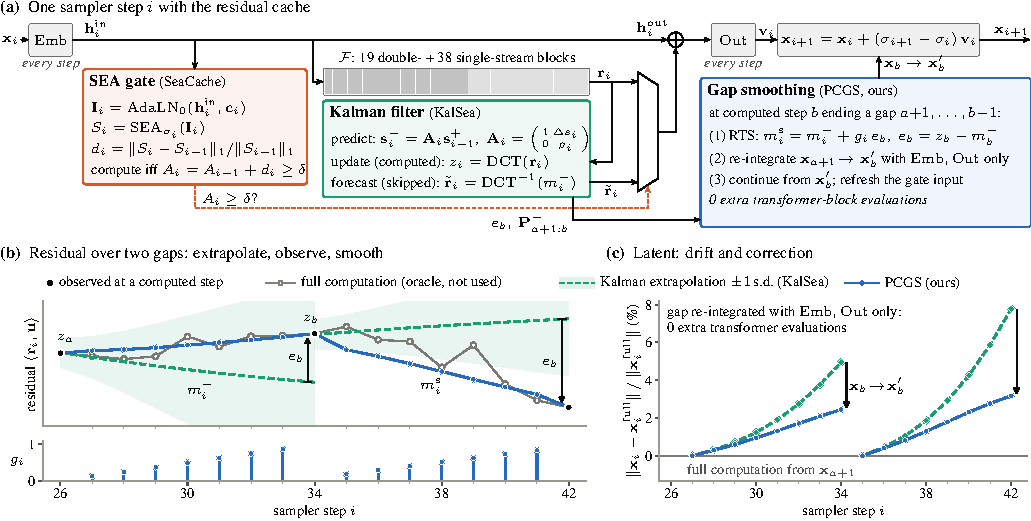
\includegraphics[width=\textwidth]{figures/method.pdf}
%     % Draft caption for the method figure (Fig. 2).  Usage in sections/method.tex:
%   \begin{figure*}[t]\centering
%     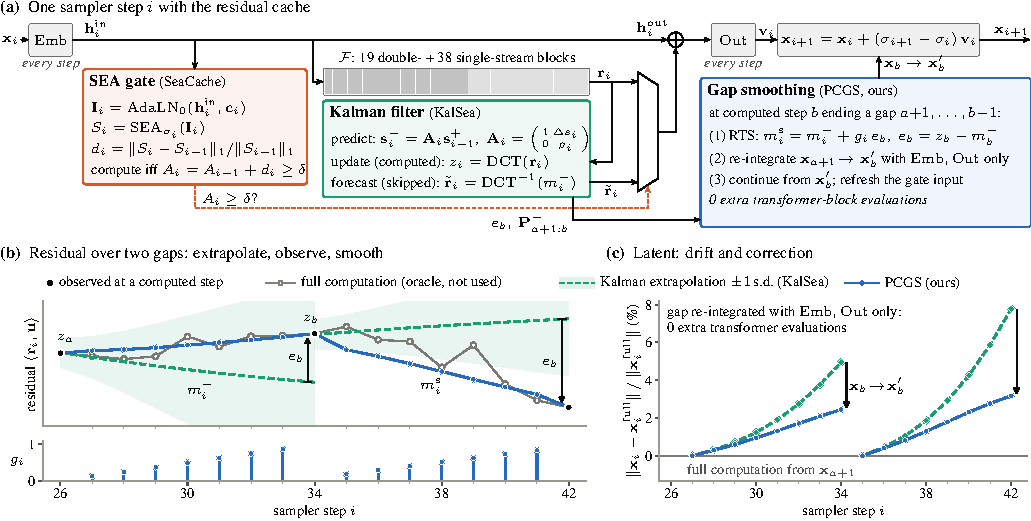
\includegraphics[width=\textwidth]{figures/method.pdf}
%     % Draft caption for the method figure (Fig. 2).  Usage in sections/method.tex:
%   \begin{figure*}[t]\centering
%     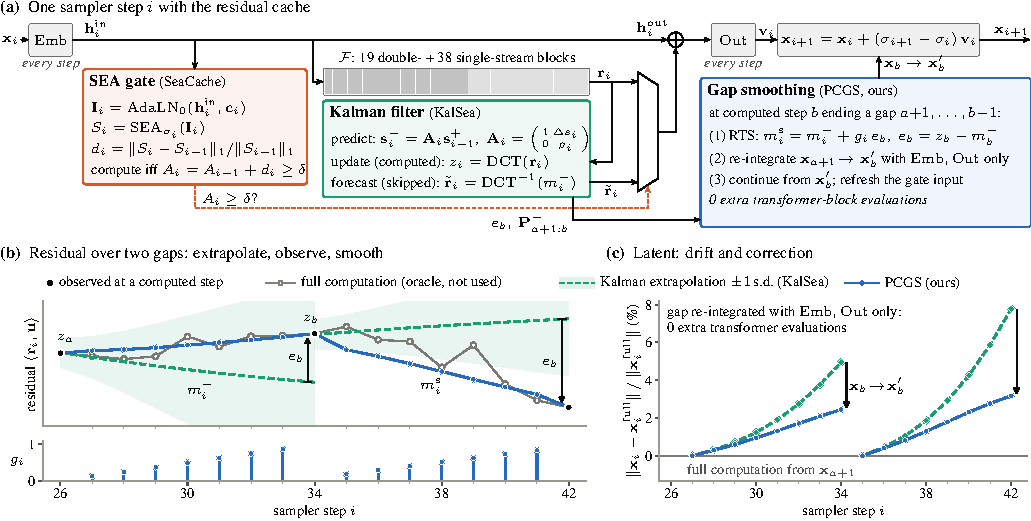
\includegraphics[width=\textwidth]{figures/method.pdf}
%     \input{figures/method_caption}
%   \end{figure*}
% Source and data: figures/src/method/ (build.sh).  Numbers below come from data/method_trace_summary.json
% (one real FLUX.1-dev generation, DrawBench prompt index 154, delta = 0.6, seed = 154).  Steps are 1-based (i = 1..N).
\caption{\textbf{Overview.}
\textbf{(a)}~In each sampler step~$i$, the \sea gate of \seacache accumulates the \sea-filtered relative $\ell_1$ change
$\gdist_i$ of the first block's modulated input and runs the transformer blocks $\blocks$ only when the accumulated change
reaches~$\delta$ (which resets it); the residual $\res_i=\blocks(\hin_i)-\hin_i$ of a computed step updates a damped-trend
Kalman filter per DCT coefficient (\kalsea), whose forecast $\resf_i$ replaces $\res_i$ on skipped steps, while $\Emb$
and $\Out$ run at every step.
\textbf{(b)}~When a computed step~$b$ ends the gap $a{+}1,\dots,b{-}1$, \pcgs propagates the innovation $e_b$ back into
the gap with the RTS gains $g_i$, which grow toward~$b$, so that the smoothed residuals $\smooth{m}_i$ replace the
extrapolation $\prior{m}_i$.
\textbf{(c)}~The gap is then re-integrated from $\lat_{a+1}$ with $\Emb$ and $\Out$ only and sampling continues from $\lat_b'$,
which roughly halves the latent deviation from full computation at~$b$ (here $5.0\%\to2.4\%$ and $7.8\%\to3.2\%$;
25--59\% lower in all ten gaps of this sample) at zero extra transformer evaluations.
Panels (b) and (c) show one real \flux generation at $\delta=0.6$ (13 of 50 steps computed) for the DrawBench prompt
whose PSNR gains (\kalsea over \seacache, \ours over \kalsea) are closest to the benchmark means (``McDonalds Church.'');
the residual is projected onto a fixed random unit direction~$\mathbf{u}$ in the lowest DCT band, which holds 89\% of the
residual energy, and the gray full-computation values come from extra evaluations made only for this figure.}
\label{fig:method}

%   \end{figure*}
% Source and data: figures/src/method/ (build.sh).  Numbers below come from data/method_trace_summary.json
% (one real FLUX.1-dev generation, DrawBench prompt index 154, delta = 0.6, seed = 154).  Steps are 1-based (i = 1..N).
\caption{\textbf{Overview.}
\textbf{(a)}~In each sampler step~$i$, the \sea gate of \seacache accumulates the \sea-filtered relative $\ell_1$ change
$\gdist_i$ of the first block's modulated input and runs the transformer blocks $\blocks$ only when the accumulated change
reaches~$\delta$ (which resets it); the residual $\res_i=\blocks(\hin_i)-\hin_i$ of a computed step updates a damped-trend
Kalman filter per DCT coefficient (\kalsea), whose forecast $\resf_i$ replaces $\res_i$ on skipped steps, while $\Emb$
and $\Out$ run at every step.
\textbf{(b)}~When a computed step~$b$ ends the gap $a{+}1,\dots,b{-}1$, \pcgs propagates the innovation $e_b$ back into
the gap with the RTS gains $g_i$, which grow toward~$b$, so that the smoothed residuals $\smooth{m}_i$ replace the
extrapolation $\prior{m}_i$.
\textbf{(c)}~The gap is then re-integrated from $\lat_{a+1}$ with $\Emb$ and $\Out$ only and sampling continues from $\lat_b'$,
which roughly halves the latent deviation from full computation at~$b$ (here $5.0\%\to2.4\%$ and $7.8\%\to3.2\%$;
25--59\% lower in all ten gaps of this sample) at zero extra transformer evaluations.
Panels (b) and (c) show one real \flux generation at $\delta=0.6$ (13 of 50 steps computed) for the DrawBench prompt
whose PSNR gains (\kalsea over \seacache, \ours over \kalsea) are closest to the benchmark means (``McDonalds Church.'');
the residual is projected onto a fixed random unit direction~$\mathbf{u}$ in the lowest DCT band, which holds 89\% of the
residual energy, and the gray full-computation values come from extra evaluations made only for this figure.}
\label{fig:method}

%   \end{figure*}
% Source and data: figures/src/method/ (build.sh).  Numbers below come from data/method_trace_summary.json
% (one real FLUX.1-dev generation, DrawBench prompt index 154, delta = 0.6, seed = 154).  Steps are 1-based (i = 1..N).
\caption{\textbf{Overview.}
\textbf{(a)}~In each sampler step~$i$, the \sea gate of \seacache accumulates the \sea-filtered relative $\ell_1$ change
$\gdist_i$ of the first block's modulated input and runs the transformer blocks $\blocks$ only when the accumulated change
reaches~$\delta$ (which resets it); the residual $\res_i=\blocks(\hin_i)-\hin_i$ of a computed step updates a damped-trend
Kalman filter per DCT coefficient (\kalsea), whose forecast $\resf_i$ replaces $\res_i$ on skipped steps, while $\Emb$
and $\Out$ run at every step.
\textbf{(b)}~When a computed step~$b$ ends the gap $a{+}1,\dots,b{-}1$, \pcgs propagates the innovation $e_b$ back into
the gap with the RTS gains $g_i$, which grow toward~$b$, so that the smoothed residuals $\smooth{m}_i$ replace the
extrapolation $\prior{m}_i$.
\textbf{(c)}~The gap is then re-integrated from $\lat_{a+1}$ with $\Emb$ and $\Out$ only and sampling continues from $\lat_b'$,
which roughly halves the latent deviation from full computation at~$b$ (here $5.0\%\to2.4\%$ and $7.8\%\to3.2\%$;
25--59\% lower in all ten gaps of this sample) at zero extra transformer evaluations.
Panels (b) and (c) show one real \flux generation at $\delta=0.6$ (13 of 50 steps computed) for the DrawBench prompt
whose PSNR gains (\kalsea over \seacache, \ours over \kalsea) are closest to the benchmark means (``McDonalds Church.'');
the residual is projected onto a fixed random unit direction~$\mathbf{u}$ in the lowest DCT band, which holds 89\% of the
residual energy, and the gray full-computation values come from extra evaluations made only for this figure.}
\label{fig:method}

%   \end{figure*}
% Source and data: figures/src/method/ (build.sh).  Numbers below come from data/method_trace_summary.json
% (one real FLUX.1-dev generation, DrawBench prompt index 154, delta = 0.6, seed = 154).  Steps are 1-based (i = 1..N).
\caption{\textbf{Overview.}
\textbf{(a)}~In each sampler step~$i$, the \sea gate of \seacache accumulates the \sea-filtered relative $\ell_1$ change
$\gdist_i$ of the first block's modulated input and runs the transformer blocks $\blocks$ only when the accumulated change
reaches~$\delta$ (which resets it); the residual $\res_i=\blocks(\hin_i)-\hin_i$ of a computed step updates a damped-trend
Kalman filter per DCT coefficient (\kalsea), whose forecast $\resf_i$ replaces $\res_i$ on skipped steps, while $\Emb$
and $\Out$ run at every step.
\textbf{(b)}~When a computed step~$b$ ends the gap $a{+}1,\dots,b{-}1$, \pcgs propagates the innovation $e_b$ back into
the gap with the RTS gains $g_i$, which grow toward~$b$, so that the smoothed residuals $\smooth{m}_i$ replace the
extrapolation $\prior{m}_i$.
\textbf{(c)}~The gap is then re-integrated from $\lat_{a+1}$ with $\Emb$ and $\Out$ only and sampling continues from $\lat_b'$,
which roughly halves the latent deviation from full computation at~$b$ (here $5.0\%\to2.4\%$ and $7.8\%\to3.2\%$;
25--59\% lower in all ten gaps of this sample) at zero extra transformer evaluations.
Panels (b) and (c) show one real \flux generation at $\delta=0.6$ (13 of 50 steps computed) for the DrawBench prompt
whose PSNR gains (\kalsea over \seacache, \ours over \kalsea) are closest to the benchmark means (``McDonalds Church.'');
the residual is projected onto a fixed random unit direction~$\mathbf{u}$ in the lowest DCT band, which holds 89\% of the
residual energy, and the gray full-computation values come from extra evaluations made only for this figure.}
\label{fig:method}
